\section{Apache Http Server}

\subsection{Historique}
%Yann

\begin{frame}
	\frametitle{De 1995 à aujourd'hui}
	\begin{itemize}
		\item 1995 : Version 1.0
		    \begin{itemize}
			\item collection de correctifs et d'additions au serveur NCSA HTTPd 1.3 : \og{} a patchy server \fg{}
		    \end{itemize}
        ~\\~\\
		\item 1999 : Fondation Apache
		    \begin{itemize}
		    	\item développe des logiciels open source sous la licence Apache (OpenOffice, Hadoop, Tomcat...)
		    \end{itemize}
	~\\~\\
		\item 2004 : Version 2.0
		    \begin{itemize}
		    	\item support de plusieurs plates-formes (Windows, Linux et UNIX, entre autres), support de processus légers UNIX, nouvelle API et support IPv6.
		    \end{itemize}

	\end{itemize}
\end{frame}

\begin{frame}
	\frametitle{Aujourd'hui}
	\begin{itemize}
		\item En janvier 2012, Apache Http server est toujours le serveur Web le plus populaire sur le marché.
	\end{itemize}
	\begin{center}
		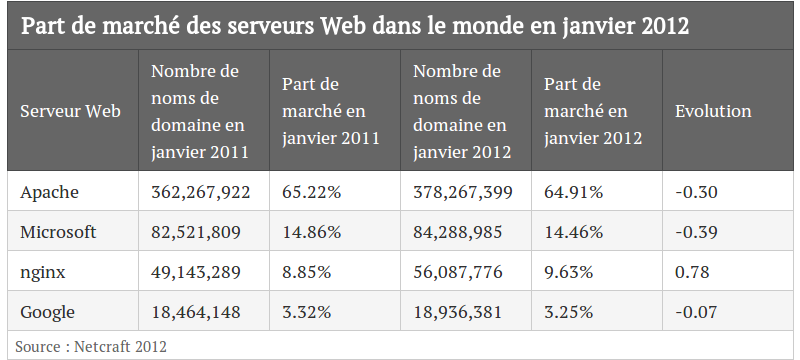
\includegraphics[scale=0.3]{Images/parts-marche.png}
	\end{center}
\end{frame}

\subsection{Fonctionnement}

\begin{frame}
	\frametitle{Fonctionnement (1/3)}
	\begin{itemize}
		\item On appelle \og{} serveur Web \fg{} à la fois le matériel informatique et le serveur Http.
	\end{itemize}
	\begin{center}
		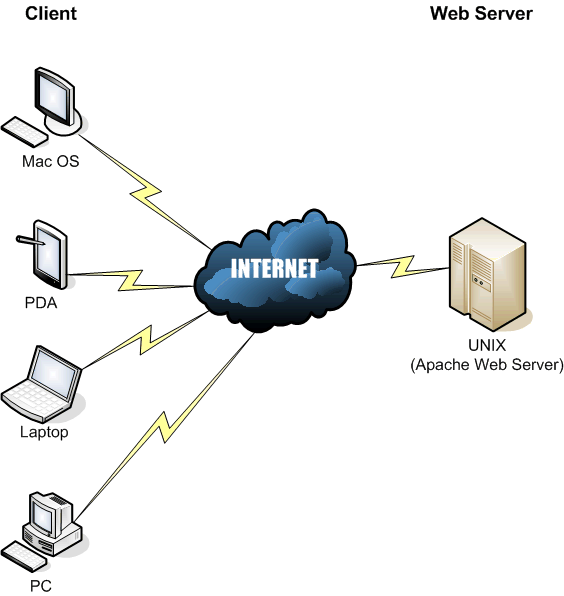
\includegraphics[scale=0.25]{Images/nuage-apache.png}
	\end{center}
\end{frame}

\begin{frame}
	\frametitle{Fonctionnement (2/3)}
	\begin{itemize}
		\item Le serveur Http attend des requêtes Http et répond en envoyant au client la page web désirée.
	\end{itemize}
	\begin{center}
		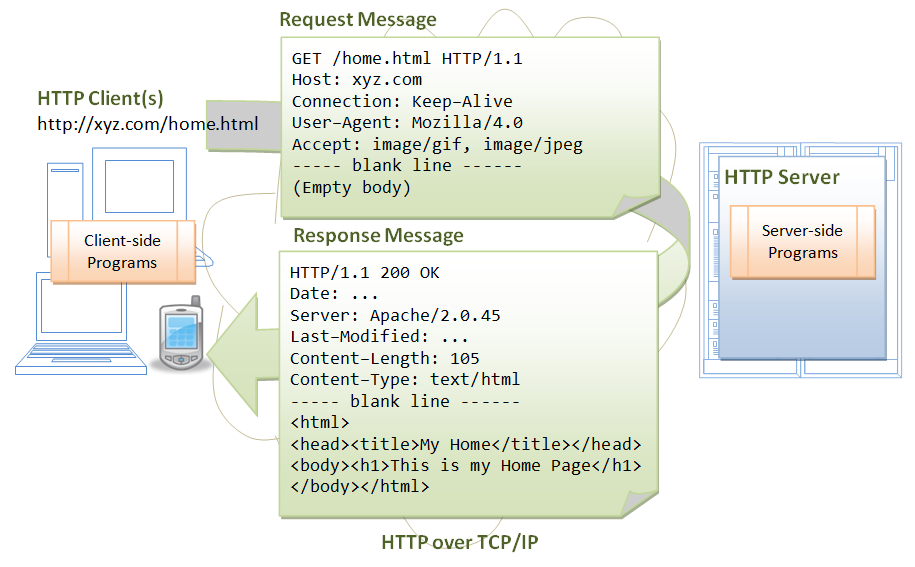
\includegraphics[scale=0.3]{Images/protocole_http.png}
	\end{center}
\end{frame}

\begin{frame}
	\frametitle{Fonctionnement (3/3)}
	\begin{itemize}
		\item Le traitement des requêtes Http par le serveur Apache se fait en plusieurs étapes.
	\end{itemize}
	\begin{center}
		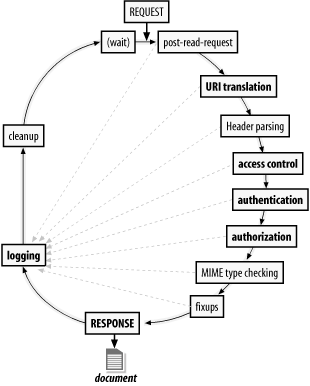
\includegraphics[scale=0.4]{Images/processing_apache.png}
	\end{center}
\end{frame}

\subsection{Fichiers de configuration}

\begin{frame}
	\frametitle{Fichiers de configuration (1/3)}
	\begin{itemize}
		\item Les fichiers de configuration se trouvent dans /etc/apache2
	\end{itemize}
	\begin{center}
		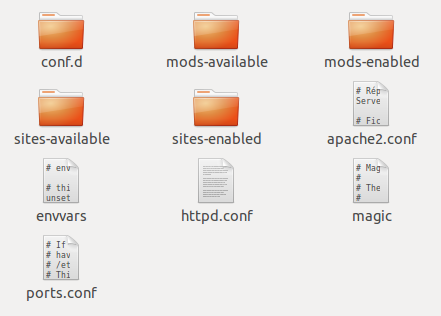
\includegraphics[scale=0.3]{Images/fichiers_config.png}
	\end{center}
\end{frame}

\begin{frame}
	\frametitle{Fichiers de configuration (2/3)}
	\begin{itemize}
	      \item Apache2.conf
	      \begin{itemize}
		  \item Ce fichier est le fichier de configuration de base. Il inclut tous les autres fichiers de configuration.
	      \end{itemize}
	      \item Ports.conf
	      \begin{itemize}
		  \item Il contient la spécification des interfaces sur lesquelles Apache écoutera les requêtes.
	      \end{itemize}
	\end{itemize}
	\begin{center}
		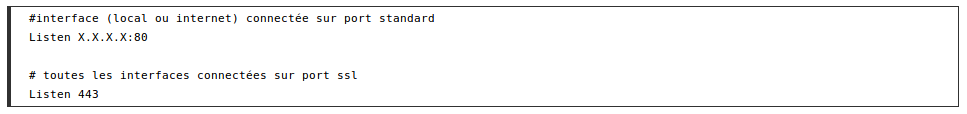
\includegraphics[scale=0.3]{Images/ports.png}
	\end{center}
\end{frame}

\begin{frame}
	\frametitle{Fichiers de configuration (3/3)}
	\begin{itemize}
	      \item Sites-available
	      \begin{itemize}
		  \item Ce dossier contient différents \textit{virtual hosts}. Il permet de définir plusieurs sites sur une même machine. Par exemple, on peut définir des sous-domaines (ex : machin.domain.tld), ainsi que d'autres domaines (ex : autredomain.tld). Les sites activés sont placés dans le dossier sites-enabled.
	      \end{itemize}
	\end{itemize}
	\begin{center}
		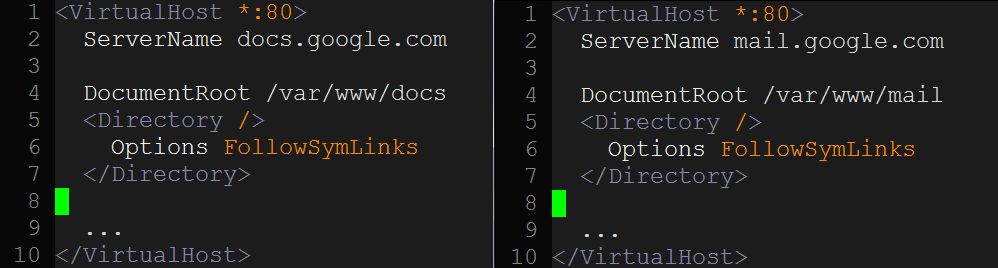
\includegraphics[scale=0.4]{Images/sites-available.png}
	\end{center}
\end{frame}

\subsection{Les modules}

\begin{frame}
	\frametitle{Les modules}
	\begin{itemize}
	  \item Il est possible d'ajouter des modules à apache, ajoutant ainsi des fonctionnalités au serveur web. Ces modules sont dans le dossier \textit{mods-available}.
	  \item On exécute le fichier .load correspondant à un module pour charger celui-ci. Le module apparaît alors dans le dossier \textit{mods-enabled}.
	  \item Lors du TP, nous utiliserons le module \textit{mod\_actions}. Celui-ci possède une directive \textit{Action} qui permet d'exécuter des scripts CGI lorsqu'un certain type de contenu MIME est requis.
	\end{itemize}
\end{frame}

